%%=============================================================================
%% Inleiding
%%=============================================================================

\chapter{\IfLanguageName{dutch}{Inleiding}{Introduction}}
\label{ch:inleiding}

De inleiding van deze scriptie licht de probleemstelling en onderzoeksvraag toe. Verder wordt de titel opgedeeld in verschillende delen. Elk deel wordt kort toegelicht om een algemene kijk te krijgen op wat de scriptie inhoudelijk bevat.\\

\section{\IfLanguageName{dutch}{Probleemstelling}{Problem Statement}}
\label{sec:probleemstelling}

Het onderzoek is van meerwaarde voor elke React frontend web developer, zowel zelfstandig als binnen een onderneming. De developers kunnen het onderzoek gebruiken als toevoeging tijdens of vooraf het ontwikkelen van een React web applicatie. Op grotere schaal is het ook interessant voor ondernemingen, in het bijzonder start-ups, maar ook \gls{kmo}'s. De onderwerpen die onderzocht worden zijn van belang voor elk jong en/of nieuw startend team.\\
Dit wilt niet zeggen dat het geen meerwaarde kan bieden voor bijvoorbeeld backend developers, mobile developers of software architecten. Het is in belang van elk die interesse heeft in React frontend web development.

\section{\IfLanguageName{dutch}{Onderzoeksvraag}{Research question}}
\label{sec:onderzoeksvraag}

De kernvraag van deze scriptie: Hoe performantie op frontend niveau op een doelgerichte en innovatieve manier verbeteren in React web applicaties?\\
Performantie is een gegeven dat in de loop der jaren in de software wereld enorm op de voorgrond is gekomen. Met hoe snel technologie en software zich ontwikkeld is het moeilijk voor iedere software ontwikkelaar om bij te houden wat de best practices zijn op het gebied van performantie. In deze `modern age` is het vanzelfsprekend dat webpagina's en apps binnen de twee seconden reageren op interactie van de gebruiker. Uit het artikel van~\textcite{Mazaika2017} leiden we af dat de vraag naar developers en software bedrijven enorm toeneemt. Dit ten gevolge van de exponentiële groei in de vraag naar webapplicaties, mobiele applicaties en andere software. Elke dag worden zij op de proef gesteld om aan de noden van gebruikers te voldoen. Met de druk van steeds meer uitgebreide en evenement rijke gebruikersomgevingen is het noodzakelijk om stil te staan bij performantie.\\
Hoe meten we performantie? Welke oplossingen biedt React ons? Waar hangt performantie van af in webapplicaties? Wat zijn de veel voorkomende valkuilen? Bestaan er ondersteunende software? Welke innovatieve technieken kunnen we toepassen? Kunnen we een leidraad vormen voor frontend performantie binnen React web applicaties?

\section{\IfLanguageName{dutch}{Javascript}{Javascript}}
\label{sec:javascript}

De taal werd gecreëerd door Brendan Eich in 1995 in zijn tijd als werknemer bij Netspace Communications, zoals aangegeven in het artikel van ~\textcite{Aston2015}. In 1997 werd het een \gls{ecma} standaard en nu behoort het tot één van de meest gebruikte programmeertalen voor het web. Zoals de naam al vrijgeeft behoort javaScript tot de scripttalen, elke scripttaal is een programmeertaal in zijn eigen recht. Voorbeelden zijn: Node js, bash, Ruby, Perl, Python, \dots\\
Scripttalen worden veel gebruikt omdat ze eenvoudig, flexibel en gebruiksvriendelijk zijn. Het zijn talen geschreven voor een run-time omgeving en worden samen met de executie van de applicatie uitgevoerd. Ze moeten niet gecompileerd worden door een compiler.\\
JavaScript wordt veel gebruikt als client side programmeertaal. Alle geschreven javaScript documenten worden bij het navigeren naar een webpagina samen met alle \gls{html} en \gls{css} documenten opgehaald van de server. Alle geïmporteerde documenten worden daarna door de browser geïnterpreteerd aan de kant van de gebruiker.

\subsection{\IfLanguageName{dutch}{JavaScript-framework}{JavaScript-framework}}
\label{sec:jsFrameworks}

Frameworks bezorgen de programmeur een duidelijke structuur en gestandaardiseerde code. Telkens opnieuw code moeten opbouwen en schrijven rooft tijd en productiviteit. Afhankelijk op welk niveau de programmeertaal wordt gebruikt bestaan er 2 typen frameworks, frontend en backend.\\
Door de immense opkom van webapplicaties begin jaren 2000 werd de vraag naar javaScript en \gls{ajax} enorm groot. Het vraag overschot zorgde voor de onvermijdelijke behoefte aan javaScript-frameworks. De frameworks brengen een oplossing voor de problemen die zuivere javaScript vormt:

\begin{itemize}[label={}]
  \item \textbf{Browserafhankelijkheid}:
  JavaScript zelf is niet afhankelijk van de browser, maar er worden wel \gls{dom} manipulaties gedaan via javaScript. De \gls{dom} is wel afhankelijk van de browser. Er moet op basis van de browser extra code voorzien worden. \newline
  \item \textbf{Prototype programmeren}:
  Maakt geen gebruik van klassen. Er wordt een prototype gemaakt van een object dat kan dienen voor overerving, het heeft limieten. \newline
   \item \textbf{Geen code herbruikbaarheid}:
  De code kan niet op een functionele manier worden gebundeld voor hergebruik, wat noodzakelijk is wanneer de complexiteit toeneemt.
\end{itemize}

Voorbeelden van \gls{js}-frameworks zijn ReactJS, AngularJS, vue.js, Ember.js, \dots

\subsection{\IfLanguageName{dutch}{Javascript library}{Javascript library}}
\label{sec:jsLibrary}

Libraries zijn een geheel van voorgeprogrammeerde functies die kunnen gebruikt worden om een aanvulling te bieden tot de reeds beschikbare functionaliteiten die het framework in kwestie aanbied. Het aspect dat ze een aanvulling bieden maakt het development eenvoudiger en makkelijker uit te breiden. In deze tijd is het simpel om een library te gebruiken met een installatie via de package manager, daarna enkel nog een import om deze in scope te plaatsen. In figuur~\ref{fig:libraryImport} op pagina~\pageref{fig:libraryImport} wordt de \textit{styled} library geïmporteerd voor het stylen van \gls{html} elementen.\\
Sommige libraries worden aanzien als een eigen framework omdat zij full-stack capaciteiten hebben, wat wil zeggen dat ze zowel frontend als backend functionaliteiten voorzien.\\
ReactJS is één van zo'n frameworks. Meningen verschillen over de interpretatie, maar beide kunnen geaccepteerd worden met elk juiste gegronde argumenten. Mensen uit de branche zoals Tom Dale, Senior Staff Software Engineer bij LinkedIn en co-creator van Ember.js, verwijzen naar React als een framework waar en tegen de online documentatie van React het als een library omschrijft.

\begin{figure}[h!]
    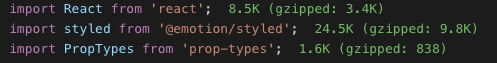
\includegraphics[width=\linewidth]{ReactInScope.png}
    \caption{Importeren van een library}
    \label{fig:libraryImport}
\end{figure}

\section{\IfLanguageName{dutch}{Frontend}{Frontend}}
\label{sec:frontend}

De letterlijke vertaling van het woord is `voorkant`, duidend op datgene wat rechtstreeks binnen de visuele waarneming valt. Alles waar de gebruiker een interactie mee kan hebben wordt aanzien als frontend. Het definieert het visuele van een webapplicatie, dat wat de gebruiker werkelijk ziet en op kan inwerken. Aan de andere kant, alles wat de gebruiker niet ziet of waarneemt wordt naar verwezen als de backend. \\
Het belang van een goede frontend is een prioriteit voor elk nieuw web project. Voor en in de loop van het project wordt er een \gls{ux}-ontwerp gemaakt, afgestemd door een bijhorend onderzoek en voor opgestelde requirements.

\begin{figure}[h!]
    \tikz\node [drop shadow={
             shadow scale=0.98,
            shadow xshift=0ex,
            shadow yshift=0ex,
            opacity=0.2,
        }]
        {\fcolorbox{black}{white}{
\includegraphics[width=\linewidth]{Frontend.png}}};
    \caption{Frontend webpagina}
    \label{fig:frontend}
\end{figure}

\section{\IfLanguageName{dutch}{Perfomantie}{Performance}}
\label{sec:performantie}

Om een duidelijk beeld te krijgen van website kwaliteit worden verschillende criteria gebruikt, performantie is hier één van. Het is een maatstaf voor laadtijden van een website die bepalen hoe snel gebruikers de \gls{ui} te zien krijgt en er iets mee kunnen doen.\\
De attentiespanne van mensen op het \gls{www} is progressief gedaald met de tijd, wat te maken heeft met de verandering in cultuur en technologie. In het artikel van~\textcite{Carette2011} worden er wetenschappelijke resultaten aangehaald die hierop duiden. De onderzoeken tonen aan dat laadtijden van enorm belang zijn voor de perceptie van mensen wanneer ze voor het eerst naar een bepaalde webpagina surfen. Het artikel beschrijft hoe een slechte laadtijd kan leiden tot imago schade, verlies van cliënteel, winstdaling en zelfs slechte \gls{seo}.\\
De meeteenheid bij uitstek voor performantie is tijd, een cruciale factor voor online succes. Alles wat visueel aan de gebruiker wordt getoond heeft invloed op hem, zowel direct als indirect. Dusdanig is performantie een fundamenteel aspect geworden voor het opleveren van een goede \gls{ui}.

\subsection{\IfLanguageName{dutch}{Waarom performatie?}{Why performance?}}
\label{sec:whyPerformance}

Voor iets kan weerlegt worden over de daadwerkelijk te creëren performantie is het goed om stil te staan bij de impact. Bedrijven met een eigen webportaal zijn er zich van bewust dat verandering nodig is om aan de eisen van gebruikers te voldoen. Er wordt veel gezegd over performantie, maar waarom is het net zo belangrijk voor hun?

\subsubsection{\IfLanguageName{dutch}{Verkoopcijfers}{Sales}}
\label{sec:sales}

De enorme groei van het \gls{www} en dagelijkse gebruik binnen de maatschappij zorgt voor een nieuw medium voor bedrijven om hun boodschap aan het doelpubliek over te brengen. Websites zijn een vaste waarde geworden binnen het businessmodel van een onderneming. Elke bezoeker van een website kan gezien worden als een potentiële klant, afhankelijk van de aard onderneming wiens website wordt bezocht. \\
De oude technieken voor het maken van sterke feature rijke sites kunnen niet meer het verwachte resultaat bieden in een steeds evoluerende niche. Een bedrijf heeft alle belang bij het onderhouden van zijn potentiële klanten en hun de beste ervaring te bieden wanneer ze naar hun website surfen. \\
In een artikel van~\textcite{Meder2017} voor Pintrest engineering worden optimalisaties in kaart gebracht op basis van een vooraf onderzochte metriek als vertrekpunt. The Telegraph deed, zoals verklaard in het artikel van~\textcite{Palmer2016}, een inverse studie waarbij een synthetische vertraging van de laadtijd een daling aantoont van het aantal pagina bezoeken wanneer de laadtijd trager wordt.

\subsubsection{\IfLanguageName{dutch}{SEO}{SEO}}
\label{sec:seo}

Search engine optimization is een prominent begrip in de bedrijfswereld sinds iedereen steeds meer onderling verbonden is door het internet en websites een groot deel uitmaken van de omzet voor bedrijven. Het principe van \gls{seo} is om een aantal doelstellingen op te stellen voor het verbeteren van de website en zo eerder in zoekopdrachten te verschijnen van zoekmachines zoals Google, Yahoo!, Bing,\dots \\
Google maakte in 2010 bekend dat er rekening zal gehouden worden met de snelheid van een website in het Google algoritme. Wat voor bedrijven de performantie van hun website nog zo belangrijk maakt. In het artikel van~\textcite{McGee2010} over de aanpassing van het Google algoritme wordt aangetoond dat laadtijd vertragingen van meer dan een halve seconde al invloed kunnen hebben op business waarden, zoals te zien is in figuur~\ref{fig:loadTimeDelaysUserImpact} op pagina~\pageref{fig:loadTimeDelaysUserImpact}. Dit maakte het voor Google relevant genoeg om op te nemen in hun algoritme.

\begin{figure}[h!]
    \tikz\node [drop shadow={
        shadow scale=0.98,
        shadow xshift=0ex,
        shadow yshift=0ex,
        opacity=0.2,
    }]
    {\fcolorbox{black}{white}{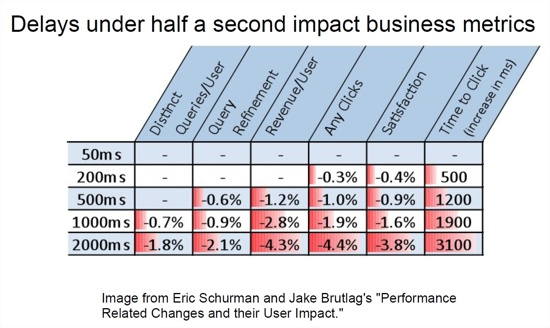
\includegraphics[width=\linewidth]{LoadTimeDelaysUserImpact.jpg}}};
    \caption{Laadtijd vertragingen met impact, Bron:~\textcite{McGee2010}}
    \label{fig:loadTimeDelaysUserImpact}
\end{figure}

\section{\IfLanguageName{dutch}{Opzet van deze bachelorproef}{Structure of this bachelor thesis}}
\label{sec:opzetBachelorproef}

% Het is gebruikelijk aan het einde van de inleiding een overzicht te
% geven van de opbouw van de rest van de tekst. Deze sectie bevat al een aanzet
% die je kan aanvullen/aanpassen in functie van je eigen tekst.

De rest van deze bachelorproef is als volgt opgebouwd:

In Hoofdstuk~\ref{ch:react} wordt React ontleed voor een goed begrip te krijgen van het framework zelf.

In Hoofdstuk~\ref{ch:theoretischePerformantie} komt het theoretische aspect van de performantie in kaart en worden de metrieken uitbundig besproken. 

In Hoofdstuk~\ref{ch:praktischePerformantie} wordt het praktische van performantie op basis van de meest courante technieken uitgewerkt.

In Hoofdstuk~\ref{ch:conclusie}, tenslotte, wordt de conclusie gegeven en een antwoord geformuleerd op de onderzoeksvragen. Daarbij wordt ook een aanzet gegeven voor toekomstig onderzoek binnen dit domein.